\documentclass[a4paper,12pt]{article}\usepackage[]{graphicx}\usepackage[]{color}
%% maxwidth is the original width if it is less than linewidth
%% otherwise use linewidth (to make sure the graphics do not exceed the margin)
\makeatletter
\def\maxwidth{ %
  \ifdim\Gin@nat@width>\linewidth
    \linewidth
  \else
    \Gin@nat@width
  \fi
}
\makeatother

\definecolor{fgcolor}{rgb}{0.345, 0.345, 0.345}
\newcommand{\hlnum}[1]{\textcolor[rgb]{0.686,0.059,0.569}{#1}}%
\newcommand{\hlstr}[1]{\textcolor[rgb]{0.192,0.494,0.8}{#1}}%
\newcommand{\hlcom}[1]{\textcolor[rgb]{0.678,0.584,0.686}{\textit{#1}}}%
\newcommand{\hlopt}[1]{\textcolor[rgb]{0,0,0}{#1}}%
\newcommand{\hlstd}[1]{\textcolor[rgb]{0.345,0.345,0.345}{#1}}%
\newcommand{\hlkwa}[1]{\textcolor[rgb]{0.161,0.373,0.58}{\textbf{#1}}}%
\newcommand{\hlkwb}[1]{\textcolor[rgb]{0.69,0.353,0.396}{#1}}%
\newcommand{\hlkwc}[1]{\textcolor[rgb]{0.333,0.667,0.333}{#1}}%
\newcommand{\hlkwd}[1]{\textcolor[rgb]{0.737,0.353,0.396}{\textbf{#1}}}%
\let\hlipl\hlkwb

\usepackage{framed}
\makeatletter
\newenvironment{kframe}{%
 \def\at@end@of@kframe{}%
 \ifinner\ifhmode%
  \def\at@end@of@kframe{\end{minipage}}%
  \begin{minipage}{\columnwidth}%
 \fi\fi%
 \def\FrameCommand##1{\hskip\@totalleftmargin \hskip-\fboxsep
 \colorbox{shadecolor}{##1}\hskip-\fboxsep
     % There is no \\@totalrightmargin, so:
     \hskip-\linewidth \hskip-\@totalleftmargin \hskip\columnwidth}%
 \MakeFramed {\advance\hsize-\width
   \@totalleftmargin\z@ \linewidth\hsize
   \@setminipage}}%
 {\par\unskip\endMakeFramed%
 \at@end@of@kframe}
\makeatother

\definecolor{shadecolor}{rgb}{.97, .97, .97}
\definecolor{messagecolor}{rgb}{0, 0, 0}
\definecolor{warningcolor}{rgb}{1, 0, 1}
\definecolor{errorcolor}{rgb}{1, 0, 0}
\newenvironment{knitrout}{}{} % an empty environment to be redefined in TeX

\usepackage{alltt}
\usepackage[applemac]{inputenc}
\usepackage[OT1,T1]{fontenc}

\setlength{\textwidth}{160mm}
\setlength{\textheight}{230mm}
\setlength{\oddsidemargin}{-5mm}
\setlength{\topmargin}{-10mm}
% \usepackage{times}
\usepackage{setspace}
\usepackage{lscape}
\usepackage{amsmath,amssymb}
\usepackage{fancyvrb}
\usepackage{multirow}
\usepackage{float}
\usepackage{hyperref}
\usepackage{color}
\usepackage{listings}
\usepackage{fancyhdr}

\usepackage{fancyvrb,moreverb,boxedminipage}

\textwidth=6in
\textheight=8in
\topmargin=0.0in
\oddsidemargin=0in 
\baselineskip=18pt
\headheight=2cm
\setcounter{MaxMatrixCols}{10}

\newcommand{\ns}{\!\!\!}
\newcommand{\e}{\varepsilon}
\newcommand{\be}{\beta}
\newcommand{\s}{\sigma}
\newcommand{\vv}{\vspace{.5cm}}
\DeclareMathOperator{\plim}{plim}
\DefineVerbatimEnvironment{code}{Verbatim}{fontsize=\small}
\DefineVerbatimEnvironment{example}{Verbatim}{fontsize=\small}

\def\by{\mathbf{y}}
\def\bx{\mathbf{x}}
\def\ba{\mathbf{a}}
\def\bb{\mathbf{b}}
\def\be{\mathbf{e}}
\def\bu{\mathbf{u}}
\def\bv{\mathbf{v}}
\def\bz{\mathbf{z}}

%===========
%Greek letter vectors
%===========
\def\bbeta{\mbox{\boldmath $\beta$}}
\def\bgamma{\mbox{\boldmath $\gamma$}}
\def\bvareps{\mbox{\boldmath $\varepsilon$}}
\def\bleta{\mbox{\boldmath $\eta$}}
\def\bmu{\mbox{\boldmath $\mu$}}
\def\btheta{\mbox{\boldmath $\theta$}}
\def\bsigma{\mbox{\boldmath $\sigma$}}
\def\blambgam{\mbox{\boldmath $\lambda_{\gamma}$}}
\def\blambbet{\mbox{\boldmath $\lambda_{\beta}$}}
\def\blambda{\mbox{\boldmath $\lambda$}}

%===========
%Matrices
%===========
\def\bX{\mathbf{X}}
\def\bY{\mathbf{Y}}
\def\bD{\mathbf{D}(\bsigma)}
\def\bV{\mathbf{V}(\bsigma)}
\def\bVinv{\mathbf{V}^{-1}(\bsigma)}
\def\bR{\mathbf{R}(\bsigma)}
\def\bA{\mathbf{A}}
\def\bB{\mathbf{B}}
\def\bZ{\mathbf{Z}}
\def\bIn{\mathbf{I_{N}}}
\def\bIm{\mathbf{I_{m}}}
\def\bIni{\mathbf{I_{n}}}
\def\SSW{\mathrm{SSW}}
\def\SSB{\mathrm{SSB}}
\def\Normal{\mathcal{N}\!}

%===========
%Parentheses, etc.
%===========
\def\op{\left(}
\def\cp{\right)}
\def\oc{\left[}
\def\cc{\right]}
\def\ok{\left\{}
\def\ck{\right\}}

%===========
%Statistical functions and real numbers.
%===========
\def\exE{\mathbb{E}}
\def\Real{\mathbb{R}}
\def\Var{\mathbb{V}ar}
\def\Proba{\mathbb{P}}

\hypersetup{colorlinks=true,linkcolor=blue,citecolor=blue, urlcolor=blue}
\urlstyle{tt}

\newenvironment{exercices}{\newcounter{moncompteur}\begin{list}
   {\bfseries Ex. \arabic{moncompteur}}{\usecounter{moncompteur}
     \setlength{\labelwidth}{2.6em}\setlength{\leftmargin}{3.1em}}}{\end{list}}
\renewcommand{\labelenumi}{\bfseries\alph{enumi})}
\newcommand{\splus}[3][0]{\texttt{>~#2}\ \ \ \ \textit{#3}\\[#1mm]}

\newenvironment{exo}
{\begin{center}\setlength{\textwidth}{140mm} \underline{Exercise:} \begin{minipage}[t]{120mm}}
{\end{minipage}\setlength{\textwidth}{160mm}\end{center}}


\usepackage{verbatim}

\lstset{ %
  language=R, 
  basicstyle=\ttfamily,
  backgroundcolor=\color{lightgray},   % choose the background color; you must add \usepackage{color} or \usepackage{xcolor}
  xleftmargin= 10 pt,
  xrightmargin= 10 pt,
  escapeinside={\%*}{*)},          % if you want to add LaTeX within your code
  frame=none,                    % adds a frame around the code
  numbers=none,                    % where to put the line-numbers; possible values are (none, left, right)
  numbersep=5pt,                   % how far the line-numbers are from the code
  numberstyle=\tiny\color{mygray}, % the style that is used for the line-numbers
  showspaces=false,                % show spaces everywhere adding particular underscores; it overrides 'showstringspaces'
}

\pagestyle{fancy}

\definecolor{mygreen}{rgb}{0,0.6,0}
\definecolor{mygray}{rgb}{0.5,0.5,0.5}
\definecolor{mymauve}{rgb}{0.58,0,0.82}
\definecolor{lightgray}{gray}{0.95}




%%%%%%%%%%%%%%%%%%%%%%%%%%%%%%%%%%%%%%%%%%%%%%%%%%%%%%%%%%%%%%%%%%%%%%%%%%%%
%
\IfFileExists{upquote.sty}{\usepackage{upquote}}{}
\begin{document}


\lhead{University of Geneva\\ \textbf{GLAM}\\
Pr. Eva Cantoni}
\rhead{GSEM\\ Spring 2022 \\ \textbf{Homework 04}}

\begin{center}
\bigskip

\bigskip

\bigskip

\bigskip

\bigskip

\bigskip

\fbox{{\Large  Two full data analysis using \texttt{glm()} - Handout}}

\bigskip

\bigskip

\bigskip
\end{center}

%%%%%%%%%%%%%%%%%%%%%%%%%%%%%%%%%%%%%%%%%%%%%%%%%%%%%%%%%%%%%%%%%%%%%%%%%%%%

% \paragraph{Course website:}\url{https://chamilo.unige.ch/home/courses/S411001/}

\setlength{\parskip}{1ex plus 0.5ex minus 0.2ex}
\parindent=0cm
\setlength{\parskip}{1ex plus 0.5ex minus 0.2ex}
\linespread{1.1}
\sloppy


\section{\underline{Exercise 1}}

% Data come from a study on infant respiratory diseases. The proportion of children developing bronchitis or pneumonia in their first year of life has been recorded by type of feeding (breast, bottle, breast with supplement) and by the newborn's sex\footnote{The GLIM
% system, C.D.Payne, Relecrre 3.77 Manual,1987}. The \verb"babyfood-bernoulli.txt" file contains the individual binary data (Bernoulli
% responses for each infant) while the file called \texttt{babyfood-binomial.txt} features grouped data (Binomial responses).



\begin{enumerate}
{\color{blue}
\item We estimate the model parameters under the two specifications (bernoulli for individual responses and binomial for grouped data) using the glm() command and store the results in the objects \texttt{baby.bern} and \texttt{baby.bin} respectively. Next, we can extract and compare the following values of interest.
\begin{itemize} 
\item The Estimates 

\begin{knitrout}
\definecolor{shadecolor}{rgb}{0.969, 0.969, 0.969}\color{fgcolor}\begin{kframe}
\begin{verbatim}
##              beta.bern   beta.bin
## (Intercept) -1.6127038 -1.6127038
## sexGirl     -0.3125528 -0.3125528
## foodBreast  -0.6692946 -0.6692946
## foodSuppl   -0.1725424 -0.1725424
\end{verbatim}
\end{kframe}
\end{knitrout}
The estimated coefficients are the same under the two specifications. 
\item The Standard Errors 
\begin{knitrout}
\definecolor{shadecolor}{rgb}{0.969, 0.969, 0.969}\color{fgcolor}\begin{kframe}
\begin{verbatim}
##             stderr.bern stderr.bin
## (Intercept)   0.1124100  0.1124100
## sexGirl       0.1410396  0.1410397
## foodBreast    0.1530057  0.1530057
## foodSuppl     0.2055847  0.2055847
\end{verbatim}
\end{kframe}
\end{knitrout}
The same goes for the standard errors. 
\item The Deviances 
\begin{knitrout}
\definecolor{shadecolor}{rgb}{0.969, 0.969, 0.969}\color{fgcolor}\begin{kframe}
\begin{verbatim}
##   dev.bern   dev.bin
## 1 1452.449 0.7219218
\end{verbatim}
\end{kframe}
\end{knitrout}

We see a difference.

\item AIC Criteria 
\begin{knitrout}
\definecolor{shadecolor}{rgb}{0.969, 0.969, 0.969}\color{fgcolor}\begin{kframe}
\begin{verbatim}
##   AIC.bern  AIC.bin
## 1 1460.449 40.23987
\end{verbatim}
\end{kframe}
\end{knitrout}

Again, we see a difference.

\item Residual Plots

\begin{knitrout}
\definecolor{shadecolor}{rgb}{0.969, 0.969, 0.969}\color{fgcolor}
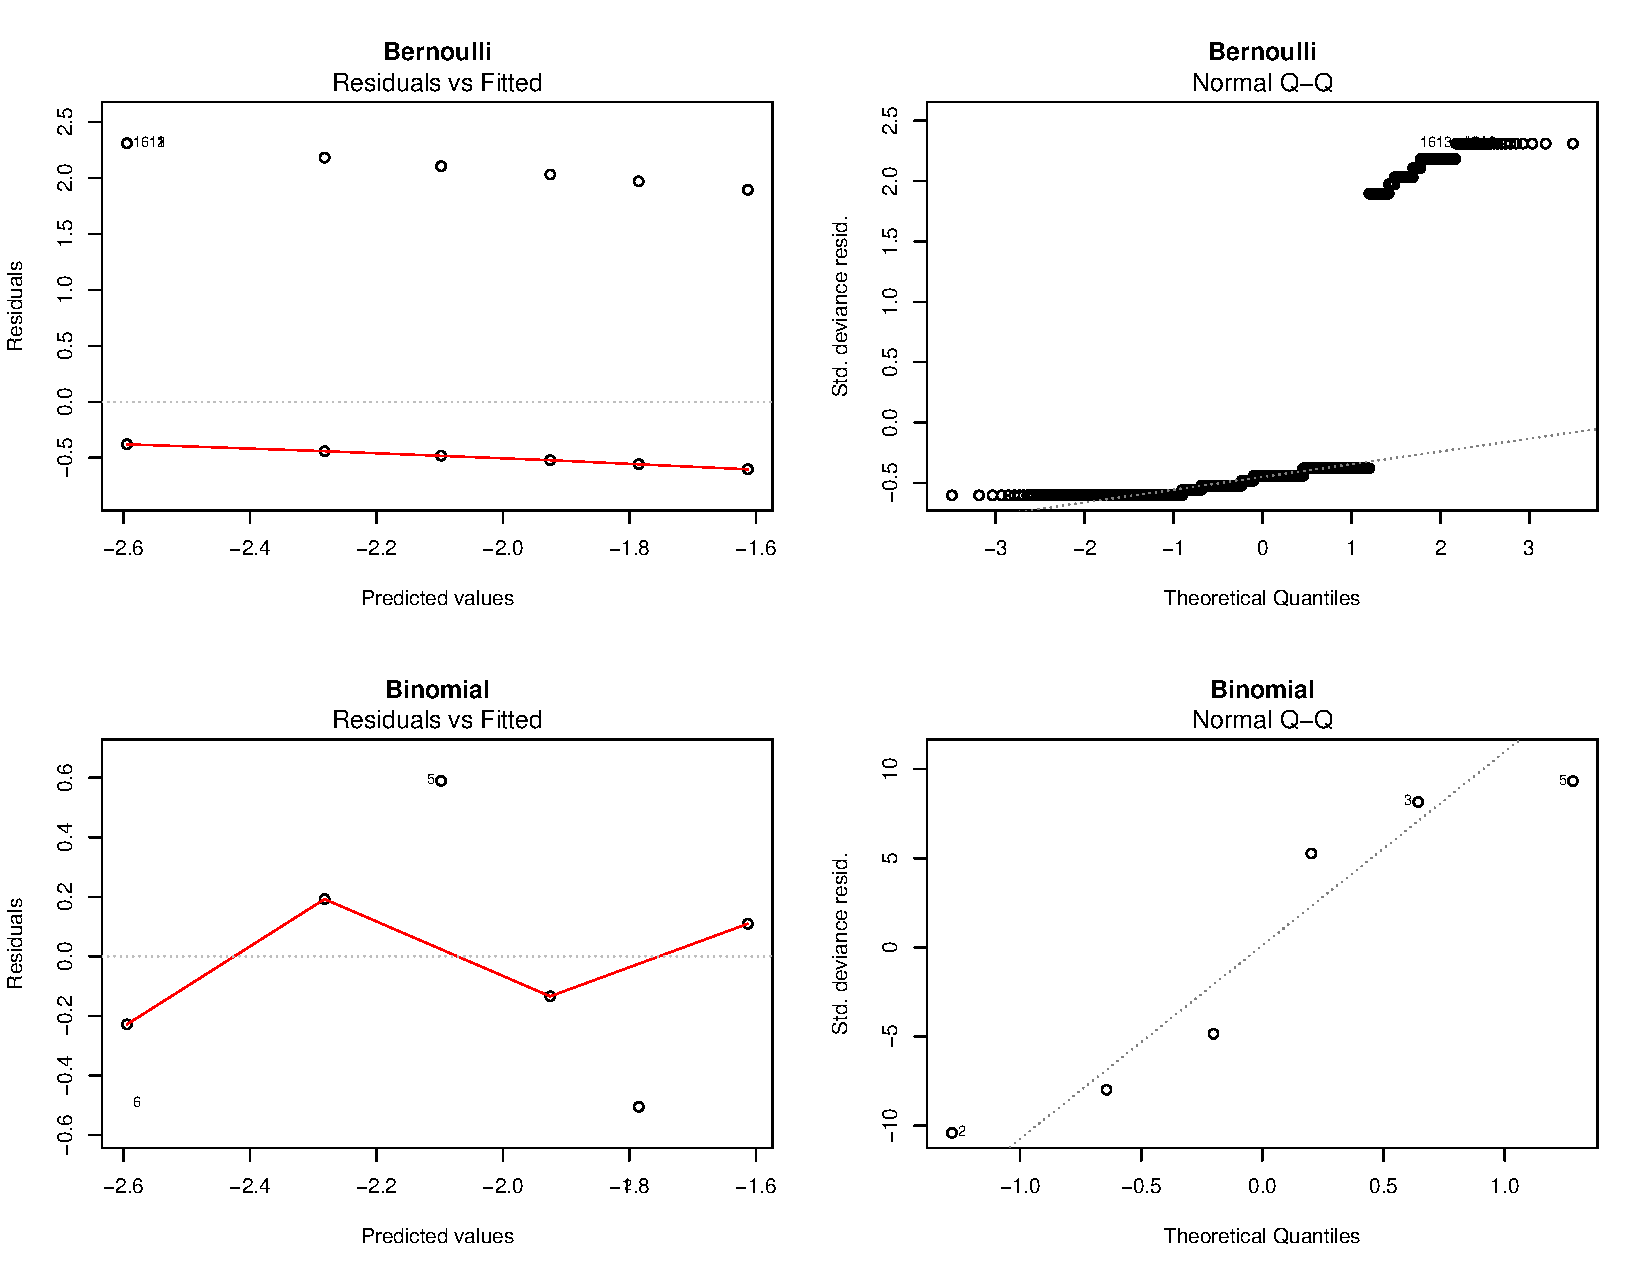
\includegraphics[width=.8\linewidth]{figure/residuals-plot} 

\end{knitrout}

Residuals present the same type of structure as we would expect using both specifications, namely, bimodality of bernoulli residuals and approximate normality for binomial.

\begin{knitrout}
\definecolor{shadecolor}{rgb}{0.969, 0.969, 0.969}\color{fgcolor}
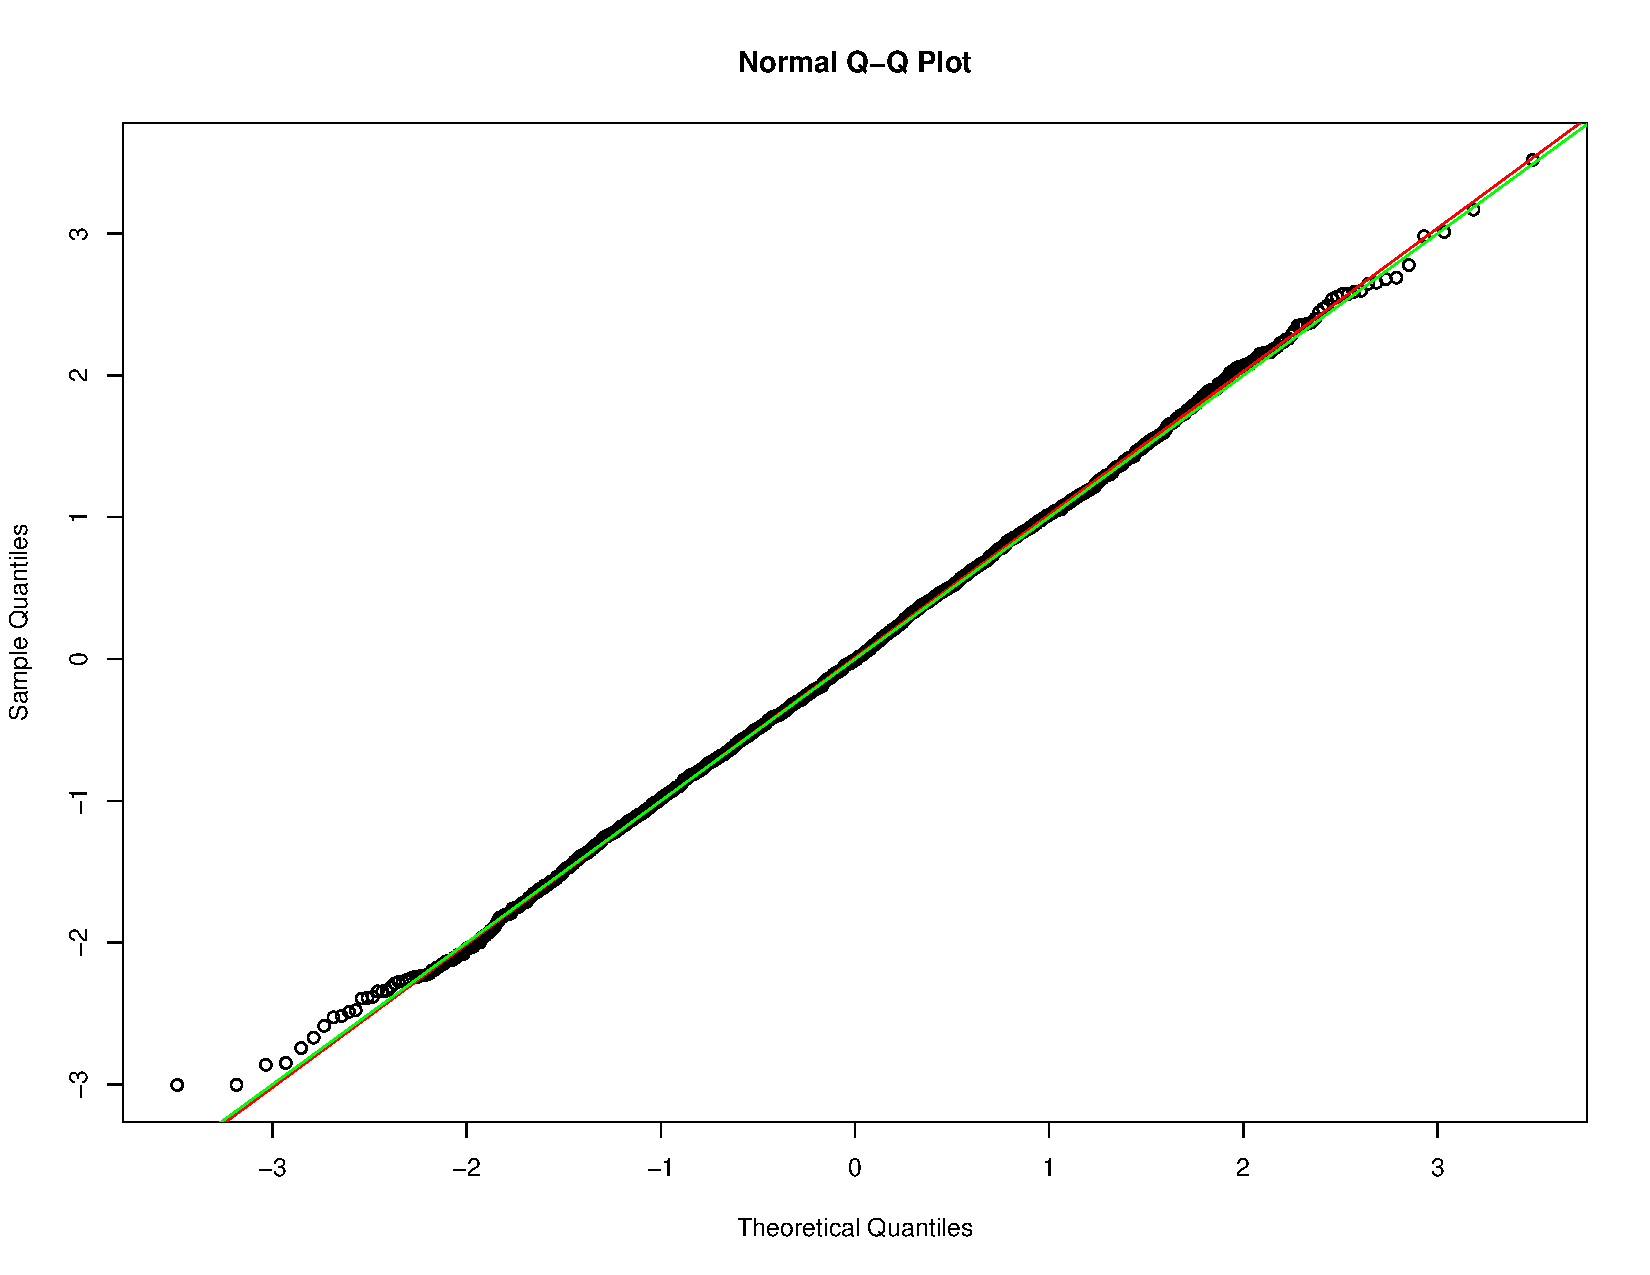
\includegraphics[width=.8\linewidth]{figure/rqr-bern} 

\end{knitrout}



\begin{knitrout}
\definecolor{shadecolor}{rgb}{0.969, 0.969, 0.969}\color{fgcolor}
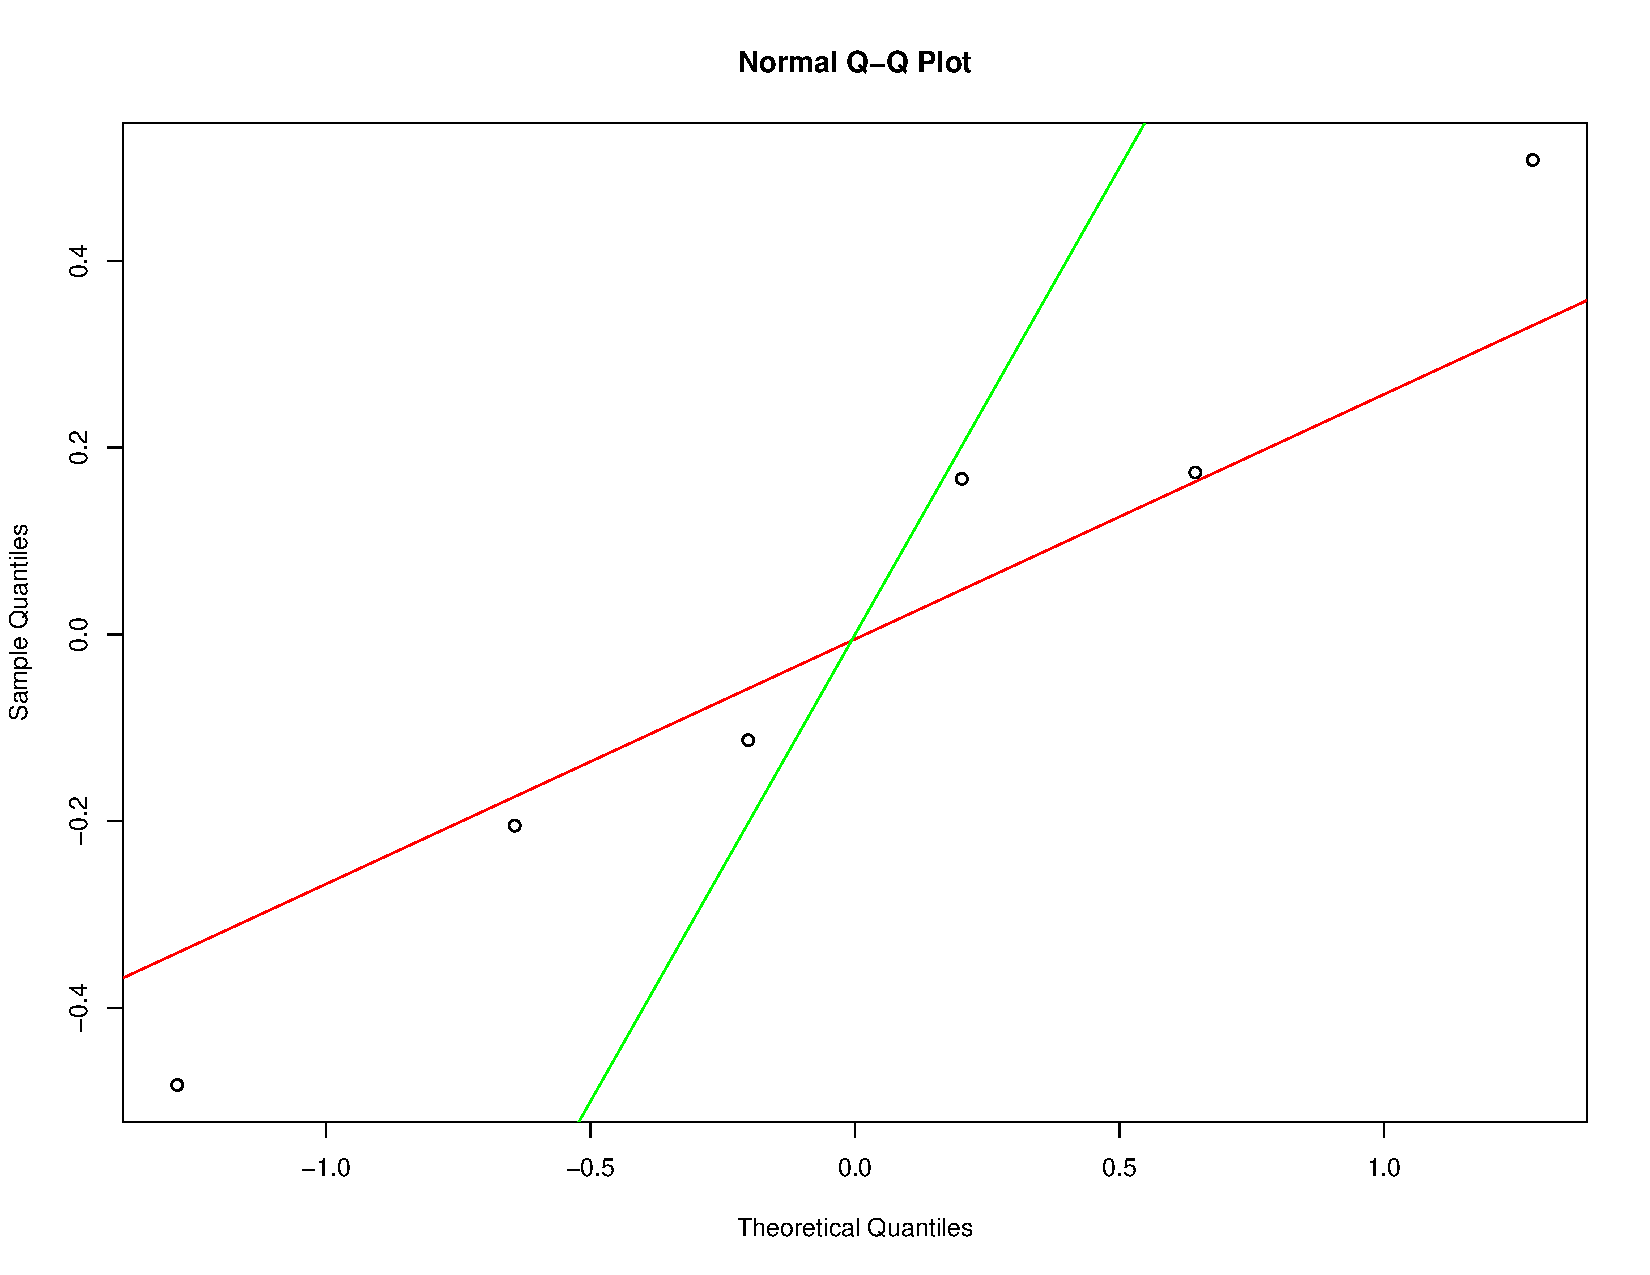
\includegraphics[width=.8\linewidth]{figure/rqr-bin} 

\end{knitrout}

By using the randomized quantile residuals, it is apparent that the fit is satisfying for the bernoulli specification. Unfortunately, given the small amount of observations in the binomial case, it is hard to see whether this fit is any good under this other specification. 

\end{itemize}
} 

\item {\color{blue}Remember that: 
\begin{enumerate}
\item\label{bernou}{$y_1,\ldots,y_n \sim \mathcal{B}(1, p_i)$, with $n=2074$,}

\begin{equation} \label{eq:ll:bernoulli}
\ell\op \bbeta ; \by | \bX \cp  = \sum_{i=1}^n y_i \log p_i + \op 1- y_i\cp \log \op 1- p_i \cp
\end{equation}

\item\label{binom}{$Y_1,\ldots,Y_6 \sim  \mathcal{B}(m_i,p_i)$ with $\sum_{i=1}^6 m_i = n = 2074$.}

\begin{equation} \label{eq:ll:binomial}
\ell\op \bbeta ; \bY | \bX \cp  = \sum_{i=1}^6 \log {m_i \choose Y_i} + Y_i \log p_i + \op m_i- Y_i\cp \log \op 1- p_i \cp
\end{equation}

Now, consider the log-likelihood for the Bernoulli model \eqref{eq:ll:bernoulli} and the grouping with respect to the six possible combinations of levels for variables \texttt{sex} and \texttt{food}: 

\begin{equation}
y_{ij} \sim \mathcal{B}\op 1, p_i \cp \ \mathrm{for} \  j =1,\dots , m_i 
\ \Rightarrow \
Y_i = \sum_{j=1}^{m_i} y_{ij} \sim \mathcal{B}\op m_i , p_i\cp
\end{equation}

We can thus rewrite, expression \eqref{eq:ll:bernoulli} as: 
\begin{align}
\ell\op \bbeta ; \by | \bX \cp  
&= \sum_{i=1}^n y_i \log p_i + \op 1- y_i\cp \log \op 1- p_i \cp\\
&= \sum_{i=1}^{6} \sum_{j=1}^{m_i} y_{ij} \log p_i + \op 1- y_{ij}\cp \log \op 1- p_i \cp\\
&= \sum_{i=1}^{6} \op\sum_{j=1}^{m_i} y_{ij}\cp \log p_i + \op\sum_{j=1}^{m_i} \op 1- y_{ij}\cp \cp \log \op 1- p_i \cp\\
&= \sum_{i=1}^{6} Y_i \log p_i + \op m_i - Y_i \cp \log \op 1- p_i \cp \\
\ell\op\bbeta ; \by | \bX \cp  
& = \ell\op\bbeta ; \bY | \bX \cp -  \sum_{i=1}^6 \log {m_i \choose Y_i}
\end{align}
\end{enumerate}

i.e. the expression of the log-likelihood of a binomial model \eqref{eq:ll:binomial} minus the term accounting for the combinatory. Since optimization is performed by derivation with respect to $\bbeta$, the score equation and its second derivative will have the same expression, yielding the same results in terms of estimates and standard errors under both specifications.
}
\item\label{compu}
{\color{blue}
The expression of the Deviance in the Bernoulli model is as follows: 
\begin{equation} \label{eq:dev:bernoulli}
\mathcal{D}^{*}\op \by, \widehat{\mathbf{p}} \cp 
= 
2 \sum_{i=1}^{2074} y_i  \log \op \frac{y_i}{\widehat{p}_i} \cp + \op 1-y_i\cp \log \op \frac{1-y_i}{1-\widehat{p}_i} \cp
\end{equation}

However, due to the nature of the data ($y_i = 0$ or $y_i = 1$), we have that $y_i\log y_i=0$ and $\op 1-y_i\cp \log \op 1 - y_i\cp = 0$, yielding the following simplifications: 

\begin{align}
\mathcal{D}^{*}\op \by, \widehat{\mathbf{p}}\cp
&=
- 2 \sum_{i=1}^{2074} y_i \log{\widehat{p}_i} + \op 1-y_i\cp  \log  \op 1-\widehat{p}_i \cp \nonumber\\
&= - 2 \sum_{i=1}^{2074} y_i \log \frac{\widehat{p}_i}{1-\widehat{p}_i} +   \log \op 1-\widehat{p}_i \cp \nonumber\\
&= - 2 \sum_{i=1}^{2074} y_i \bx_i^T\widehat{\bbeta} +   \log \op 1-\widehat{p}_i \cp \nonumber \\
\mathcal{D}^{*}\op \by, \widehat{\mathbf{p}}\cp 
&= - 2 \sum_{i=1}^{2074} \widehat{p}_i \bx_i^T\widehat{\bbeta} +  \log \op 1-\widehat{p}_i \cp  \ \mathrm{since :} \sum_{i=1}^{2074} \op y_i - \widehat{p}_i \cp \bx_i = 0 
\end{align}

From the last expression, it is apparent that, given the values of $\widehat{\bbeta}$, the deviance doesn't depend on $y_i$, making it a bad GOF measure. Consequently, it holds that the distribution of this statistic conditional on values of $\widehat{\bbeta}$ is degenerate, meaning that the approximation via the $\chi^2$ is not possible.  

In the binomial specification, this doesn't hold any more, given that $Y_i$ can have different possible values, meaning that their contributions to the residual deviance are not neglected.   

{\color{red}
\begin{equation}
\mathcal{D}^{*}\op \bY, \widehat{\mathbf{p}} \cp 
= 
2 \sum_{i=1}^6 Y_i \log \left( \frac{Y_i}{m_i \widehat{p}_i} \right) + \op m_i-Y_i\cp  \log \left( \frac{m_i- Y_i}{m_i(1-\widehat{p}_i)} \right)
\end{equation}
}
In that case, the statistic is a good GOF measure and its distribution can be approximated with the $\chi^2$. However, as in any case, the distribution of the deviance depends also on the number of available observations! Moral of the story : be careful when using the deviance in a binomial model.  
}

\item {\color{blue} The AIC criterion is based on the Log-likelihood, meaning that it could be used for model selection under both specifications. However, when used, you should be attentive on comparing two nested models.}

\end{enumerate}

\section{\underline{Exercise 2}}

{\color{blue}  Check the code for an annotated solution.}

\end{document}
